\documentclass[8pt]{article}
%%%%%%%%%%%%%%%%%%%%%%%%%%%
% Packages
%%%%%%%%%%%%%%%%%%%%%%%%%%%
\usepackage{hyperref}
\hypersetup{
  pdfauthor={Marco Arieli Herrera-Valdez},
  pdftitle={}
  pdftex,
  colorlinks=true,
  urlcolor=Bittersweet,
  linkcolor=blue,
  pdftoolbar=true,
  pdfmenubar=true,
  citecolor=Purple,
  filecolor=blue,
}
%\usepackage[spanish,es-nodecimaldot]{babel}
\usepackage{lscape}
\usepackage{setspace}
%\setstretch{1.1}
%\doublespacing
\usepackage[utf8]{inputenc}
%\usepackage[latin1]{inputenc}
%\usepackage[applemac]{inputenc}
%% Only if the base font of the document is to be different, say sans serif
% Text layout
\usepackage[T1]{fontenc}
\usepackage[scaled=0.92]{helvet}
\renewcommand*\familydefault{\sfdefault}
\usepackage{authblk}
\usepackage{graphicx}
\usepackage{python}
\usepackage{mathtools,amsfonts,amssymb,amsmath}
\usepackage[dvipsnames,svgnames,hyperref,table]{xcolor}
%\usepackage{xcolor}
\usepackage{microtype}
\usepackage{sidecap}
%\hypersetup{pdfpagemode=FullScreen}
%\usepackage[left=2.5cm,right=2.5cm,top=0cm,bottom=2cm,includehead]{geometry}
\usepackage{geometry}
\usepackage{fancyhdr}
%\pagestyle{fancyplain}
%\pagestyle{plain}
% The color packages must appear before the pdfpages package
%\usepackage{chemarr}
\usepackage{listings}
%\usepackage[normalem]{ulem}
%\usepackage[usenames,svgnames,dvipsnames]{xcolor}
%\usepackage[dvipsnames,svgnames,usenames]{xcolor}
%\usepackage{booktabs} % Top and bottom rules for table
\usepackage[font=small,labelfont=bf]{caption}
%\usepackage{wrapfig}
%\usepackage{subfigure}
%\usepackage{beamerthemesplit}
\usepackage{boldline}
\usepackage{multirow}
\usepackage{multicol}
\usepackage{longtable}
\usepackage{times}
\usepackage{animate}
\usepackage{pdfpages}
\usepackage{url}
%\usepackage{multimedia}
%\usepackage{movie15}
%\usepackage{media9}
\usepackage{verbatim}
%\usepackage{pgflibraryarrows}
%\usepackage{pgflibraryshapes}
\usepackage{tikz}
%\usetikzlibrary{arrows,shapes,matrix,chains,calc,positioning}
%\usetikzlibrary{trees,mindmap}
\usepackage{ifthen}
\usepackage{animate}

% To get the envelope in the author list
\usepackage[misc]{ifsym}
%\usepackage[misc,geometry]{ifsym}

%\Letter after the name of the corresponding author

% --------------------------------------
% Bibliography
% --------------------------------------
%\usepackage[sort&compress]{natbib}
\usepackage[round,sort&compress]{natbib}
%\usepackage[numbers,sort&compress]{natbib}
%\bibliographystyle{plainnat}

/Users/curandero/docsLaTeX/mahvLaTeXCommands.tex
\usepackage[utf8]{inputenc}
\usepackage[position=top]{subfig}
\usepackage{tkz-berge}
\usetikzlibrary{arrows,petri,topaths}
\tikzstyle{vertex}=[circle, draw, inner sep=3pt, minimum size=5pt]
\newcommand{\vertex}{\node[vertex]}
\setstretch{1.3}
%
\title{Dinámica inicial de la epidemia de Covid-19 en en mundo y en México }
\author{Marco Arieli Herrera-Valdez}
\date{April 2020}
%
\begin{document}
%
%\begin{flushleft}
%\begin{Large}
%{Estimaciones y análisis de la dinámica inicial de la mortalidad de casos epidemia de Covid-19 en México a partir de los datos mundiales}
%\end{Large}\\
%\smallskip
%\begin{large}
%Carlos Ignacio Herrera-Nolasco$^1$, Eugenia O'Reilly-Regueiro$^{4,\email}$,
%Marco Arieli Herrera-Valdez$^{1,\email}$
%\end{large}\\
%\smallskip
%$^1$ Departamento de Matemáticas, Facultad de Ciencias, Universidad Nacional Autónoma de México\\
%$^4$ Instituto de Matemáticas, Facultad de Ciencias, Universidad Nacional Autónoma de México\\
%$\email$ marcoh@ciencias.unam.mx, eugenia@im.unam.mx
%\end{flushleft}
%
% ---------------------------------------------------------
\section*{Análisis de las primeras semanas de la dinámica de la pandemia de {Covid-19} y estudio de mecanismos macroscópicos de propagación con apoyo de modelos estocásticos}
Carlos Ignacio Herrera-Nolasco, Eugenia O'Reilly-Regueiro, Sergio Iván López Ortega, Marco Arieli Herrera-Valdez.


% !TEX root = tsam_Covid19_Mexico.tex
\subsection*{Inferencia de características del curso temporal de la enfermedad de Covid-19 a partir de medidas macroscópicas basadas en reportes de casos, recuperaciones y muertes}

\paragraph{Retrasos entre comienzo de síntomas y recuperación o muerte a partir de los primeros reportes de caso en el mundo}


\paragraph{Participantes.} Carlos Ignacio Herrera-Nolasco, Eugenia O'Reilly-Regueiro, Sergio Iván López Ortega, Marco Arieli Herrera-Valdez. Este trabajo es parte de un reporte técnico que está siendo editado para su revisión por pares. Se pueden encontrar más detalles y referencias en \url{https://scab-unam.github.io/tsamCovid-19/tsam_Covid19_analysis}.  

?` Es posible observar en los reportes de casos hechos a nivel mundial indicaciones del tiempo que tarda una persona en morir por complicaciones de Covid-19 a partir comienza a tener síntomas ? Es decir, ?`es posible estimar el retraso en entre la muerte y la manifestación de síntomas desde una perspectiva macroscópica de los casos y los decesos por caso en distintos países?

La pregunta anterior puede ser contestada al considerar, el retraso entre primer reporte de casos y el primer reporte de muertes en distintos países. La mayoría de los países que primero reportaron casos también reportó muertes (sin retraso). Sin embargo, a medida que pasaron las semanas, se fue observando una tendencia que arroja un retraso promedio de 18 días entre primer caso confirmado y primera muerte en varios países (\figref{fig:reportArrivals}). Es posible medir dicha diferencia utilizando distintos métodos, entre los cuales está simplemente medir la distancia horizontal entre las gráficas acumuladas del número de países que han reportado primer caso o muerte, respectivamente (\figref{fig:reportArrivals} paneles de arriba). 
%
\begin{figure}[h]
\caption{Retrasos entre reportes de casos (arriba), muertes (en medio), y recuperaciones (abajo). }. \label{fig:reportArrivals}
\begin{minipage}{0.6\textwidth}
\includegraphics[width=\textwidth]{../tsam_Covid19_analysis/figures/tsam_Covid19_JHU_reportArrivals_AllCountries}
\end{minipage}%
\begin{minipage}{0.4\textwidth}
\includegraphics[width=\textwidth]
{../tsam_Covid19_analysis/figures/tsam_Covid19_JHU_delays_caseDeaths}
\end{minipage}%
\end{figure}
De esa forma también es posible medir el retraso entre reportes de casos y primera recuperación, que resulta ser de aproximadamente 12 días. 

\bigskip
La fatalidad en casos confirmados puede depender de una diversidad de factores como la calidad de los servicios de salud, y el acceso a dichos servicios, entre otros. 
Sin embargo, es posible observar algunas similitudes macroscópicas en el comportamiento de las defunciones por Covid-19 en lugares que podría pensarse que los fallecimientos presentarían comportamientos muy distintos , como China y Korea del Sur por un lado, o Italia, por otro. 
En Korea del Sur y China, el control es muy estricto y la cuantificación de casos ha sido masiva. 
En cambio en Italia, donde la estructura poblacional es distinta, ha habido más fallecimientos por Covid-19, y ha sido rebasado el sistema de salud al grado de tener que negar el uso de respiradores a la gente. 
Sin embargo, en los tres paises el cociente de fatalidad de casos (CFR por sus siglas en inglés) tiene muchas similitudes (\figref{fig:estimates}, panel izquierdo), que se pueden explotar para obtener las contribuciones relativas de los fallecimientos por Covid-19 (\figref{fig:reportArrivals}, panel derecho) por cada grupo de edad al total de muertes observadas, y usar esas estimaciones. 


%
\begin{figure}[h]
\caption{Estimaciones de fatalidad para México tomando en cuenta grupos de edad, con los datos de China, Korea del Sur, e Italia, calculado hasta el 11 de abril de 2020, y usando un factor de ajuste por subreporte igual a 1. }. \label{fig:estimates}
\begin{minipage}{0.6\textwidth}
\includegraphics[width=\textwidth]{../tsam_Covid19_analysis/figures/tsam_Covid19_JHU_cfr+propDeathCases_ByAge_China+SKorea+Italy_OneFigure.png}
\end{minipage}%
\begin{minipage}{0.4\textwidth}
\includegraphics[width=\textwidth]
{../tsam_Covid19_analysis/figures/tsam_Covid19_JHU_cfr+propDeathCasesByAgeTS_EstimatesMexico_subReportFactor12.png}
\end{minipage}%
\end{figure}

Por su similitud, es posible usar los pesos relativos de las defunciones de los distintos grupos de edad y  hacer distintas predicciones para el caso de México (\figref{fig:estimates_sp}).


Las proyecciones obtenidas usando los datos de los distintos países son similares. Hay que tomar en cuenta que estos datos no han sido ajustados con respecto a subreporte. Por ejemplo, sin ajustar los datos por subreporte, la estimación del 11 de abril de 2020 es  de alrededor 150 muertes de adultos de más de 70 años en México. 
Usando un factor de ajuste por subreporte igual a 10, estaríamos estimando que el número de muertes por COVID-19 en México sería aproximadamente 1500. 


Es importante mencionar que estas estimaciones no toman en cuenta la estructura poblacional en México, o la de los países tomados para el análisis, pero esa información está implícita en los datos de dichos países. 







% !TEX root = ../tsam_Covid19_Mexico/tsam_Covid19_Mexico.tex



\subsection*{Estimación de fecha de inicio y pico de la epidemia de Covid-19}
\paragraph{Participantes.} Carlos Ignacio Herrera-Nolasco, Marco Arieli Herrera-Valdez. Este trabajo es parte de un reporte técnico que está siendo editado para su revisión por pares. Se pueden encontrar más detalles y referencias en \url{https://scab-unam.github.io/tsam_Covid-19/tsam_Covid19_models/figures/Covid19_Mexico_InitialFit_Herrera-Valdez+Herrera-Nolasco_2020.png}.  

Los casos de Covid-19 se pueden dividir en distintos grupos dependiendo de la duración del periodo de carga viral, que a su vez indica su contribución potencial a la cadena de transmisión. Se puede entonces usar un modelo parecido en esencia al SIR. Sin embargo, hay que distinguir que los recuperados pueden permanecer contagiosos. Es decir, los recuperados pueden seguir participando en la cadena de infección. Para no generar confusiones en ese sentido, dividimos a la población en tres grupos de tamaños $N$, $I$, y $W$ que representan respectivamente los no infectados, infectados, y retirados de la cadena de infección \citep{Herrera}. 
\begin{eqnarray}
N(t+h) &=& N(t) - X_{NA}(t)
\\
I(t+h) &=& X_{NA}(t) + \sum{Y_{Ik}(t): k \in \lrSet{A,M,S,C}}  - D(t)
\\
W(t+h) &=& \sum_{k \in \lrSet{A,M,S,C}} Y_{Ik}(t) 
\end{eqnarray}

\begin{figure}[h] 
\includegraphics[width=\textwidth]{../tsam_Covid19_models/figures/Covid19_Mexico_InitialFit_Herrera-Valdez+Herrera-Nolasco_2020}
\caption{Estimación de la fecha de inicio y pico de la epidemia ajustando los datos iniciales de la epidemia de Covid-19 en México. La fecha cero representa el 27 de febrero de 2020. La fecha de inicio de la epidemia es aproximadamente 39 días antes, aproximadamente el 20 de enero de 2020.} \label{fig:inicioPicoNIW}
\end{figure}


Los valores esperados de los muestreos del modelo estocástico se pueden utilizar para derivar una ecuación determinista para el régimen en el que los tamaños poblacionales son grandes (Fig.~\ref{}). 
\begin{figure}[h]
\centering
\begin{minipage}{0.65\textwidth}
\begin{eqnarray*}
\partial_{t} x &=& -  \lambda x\\
\partial_{t} y &=& \lambda x - \vec{\gamma} \cdot \vec{y}  - \frac{y_{C}}{\tau_{F}}
\\
\partial_{t} w &=&\vec{\gamma} \cdot \vec{y}
\end{eqnarray*}
\end{minipage}%
\begin{minipage}{0.35\textwidth}
\centering
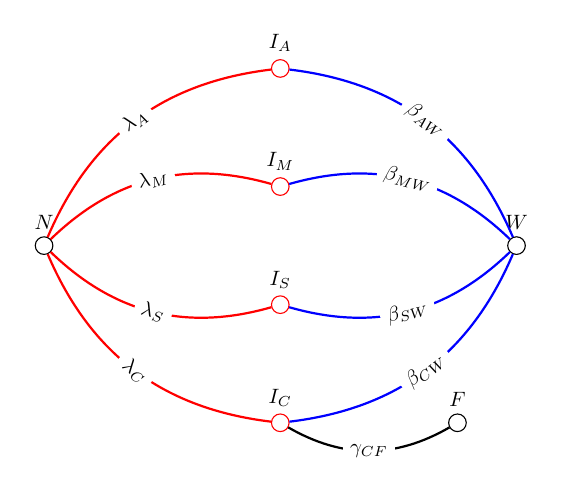
\begin{tikzpicture}[scale=0.75,transform shape]
	\vertex[label=\textcolor{black}{$N$},color=black](N) at (-4,0) { };
	\vertex[label=\textcolor{black}{$I_{A}$},color=red](A) at (0,3) {};
	\vertex[label=\textcolor{black}{$I_{M}$},color=red](M) at (0,1) {};
	\vertex[label=\textcolor{black}{$I_{S}$},color=red](S) at (0,-1) {};
	\vertex[label=\textcolor{black}{$I_{C}$},color=red](C) at (0,-3) {};
	\vertex[label=\textcolor{black}{$W$},color=black](W) at (4,0) { };
	\vertex[label=\textcolor{black}{$F$}](F) at (3,-3) {};
  \tikzstyle{LabelStyle}=[fill=white,sloped]
  \tikzstyle{EdgeStyle}=[bend left]
  \Edge[label=$\lambda_{A}$,color=red](N)(A)
  \Edge[label=$\lambda_{M}$,color=red](N)(M)
  \Edge[label=$\beta_{AW}$,color=blue](A)(W)
  \Edge[label=$\beta_{MW}$,color=blue](M)(W)
  \tikzstyle{EdgeStyle}=[bend right]
  \Edge[label=$\lambda_{S}$,color=red](N)(S)
  \Edge[label=$\lambda_{C}$,color=red](N)(C)
  \Edge[label=$\beta_{SW}$,color=blue](S)(W)
  \Edge[label=$\beta_{CW}$,color=blue](C)(W)
  \Edge[label=$\gamma_{CF}$](C)(F)
\end{tikzpicture}
\end{minipage}%
\caption{Límite determinista del modelo estocástico usado en la \figref{fig:inicioPicoNIW} para simular escenarios de la epidemia de Covid-19 en México. }
\end{figure}


\subsubsection*{Trabajo en progreso.} Continuamos desarrollando modelos estocásticos de dinámica de propagación basados en estimaciones cualitativas similares a las descritas arriba, con la intención de explicar mecanismos subyacentes a la propagación de la epidemia.  
% ---------------------------------------------------------

%\paragraph{Acknowledgments:}


\bibliographystyle{plainnat}
\bibliography{Covid19,epidemiology}
\end{document}
